\documentclass[11pt,a4paper]{article}
\usepackage[T1]{fontenc}
\usepackage[utf8]{inputenc}
\usepackage{lmodern,microtype}
\usepackage[margin=25mm]{geometry}
\usepackage{amsmath,amssymb,amsthm,booktabs,graphicx,array}
\usepackage{xcolor,tikz}
\usetikzlibrary{arrows.meta,positioning}
\definecolor{inkplum}{HTML}{573354}
\definecolor{inkteal}{HTML}{236B70}
\usepackage{hyperref}
\hypersetup{colorlinks=true,linkcolor=inkplum,citecolor=inkplum,urlcolor=inkteal,
 pdftitle={A moment obstruction and minimal-degree polynomial nonconforming Stokes elements on tetrahedra},
 pdfauthor={Anonymous}}
\usepackage{fancyhdr}
\pagestyle{fancy}\fancyhf{}
\fancyhead[L]{\small Minimal-degree moment elements on tetrahedra}
\fancyfoot[C]{\thepage}
\setlength{\headheight}{14pt}
\setlength{\parskip}{0.3em}
\setlength{\emergencystretch}{2em}
\newtheorem{theorem}{Theorem}[section]
\newtheorem{lemma}[theorem]{Lemma}
\newtheorem{proposition}[theorem]{Proposition}
\newtheorem{corollary}[theorem]{Corollary}
\newtheorem{conjecture}[theorem]{Conjecture}
\theoremstyle{definition}
\newtheorem{definition}[theorem]{Definition}
\newtheorem{example}[theorem]{Example}
\theoremstyle{remark}
\newtheorem{remark}[theorem]{Remark}
\newcommand{\M}{\mathcal M}
\newcommand{\avg}{\mathop{\mathchoice{{\textstyle\int}\mkern-15.5mu{-}\mkern2mu}{\int\mkern-12mu{-}\mkern1mu}{\int\mkern-11mu{-}}{\int\mkern-11mu{-}}}\nolimits}
\newcommand{\evid}[1]{\textsf{[#1]}}
\newcommand{\Pol}{\mathbb P}
\newcommand{\J}{J}
\title{A moment obstruction and minimal-degree polynomial\\
nonconforming Stokes elements on tetrahedra}
\author{Anonymous}
\date{22 October 2026}
\begin{document}
\maketitle

\begin{abstract}
Nonconforming finite elements for incompressible flow are often
specified by \emph{moments}: averages of the velocity against
polynomials on each face and inside each cell. A recent paper by
Balazi, Allaire, Jolivet and Omnes builds tetrahedral Stokes elements
of second and third order in this way and leaves open whether the
fourth-order element can be obtained by adding fifteen quintic
polynomials to the quartics. We show that it cannot, and we explain
why. For moments of degree \(n\) on faces and \(n-1\) in the cell, we
compute exactly which polynomials of degree \(n+2\) are invisible to
all moments: for every \(n\) they form a seven-dimensional space with an
explicit basis. Consequently degree \(n+2\) suffices only for \(n=1,2\);
for \(n\ge3\) exactly \((n-1)(n-2)/2\) moment directions are missing,
and degree \(n+3\) is necessary and sufficient. These degree statements
concern single-cell polynomial spaces that contain all polynomials of
degree \(n+1\) and are unisolvent for exactly these moments. At fourth
order the single missing direction is detected by a short symmetry
argument and supplied by the Vandermonde polynomial of the barycentric
coordinates; the result is a 50-dimensional element that does not
depend on vertex numbering. For every \(n\) we prove that numbering-free
elements using the smallest possible number of top-degree functions exist;
we give them explicitly for \(n=4,5\) and check an explicit family up to \(n=8\).
In two dimensions the analogous count shows that no extra degree is ever
needed, which explains why triangular constructions extend to all
orders. A numerical Stokes test shows rates consistent with fourth-order
convergence; the computed discrete inf-sup values are 0.40--0.37 for the
four coarsest meshes.
\end{abstract}

\noindent\textbf{MSC 2020:} 65N30 (primary); 65N12, 76D07, 33C45, 20C30.\\
\noindent\textbf{Keywords:} nonconforming finite elements; Stokes
equations; unisolvence; tetrahedral elements; Jacobi polynomials;
moment degrees of freedom.

\section{Introduction}
\label{sec:intro}

\subsection{What moment degrees of freedom are for}

A finite element is a local polynomial space together with a list of
linear functionals, the \emph{degrees of freedom}, that determine each
local function uniquely. When neighbouring cells share the degrees of
freedom attached to a common face, the pieces are glued together into a
global space. If the shared quantities are point values at vertices,
the global functions are continuous. If they are \emph{moments}, that
is, integrals \(\int_F v\,q\,ds\) against test polynomials \(q\) on a face
\(F\), the global functions may jump across faces but the jumps are
orthogonal to the tests. Such elements are called \emph{nonconforming};
the lowest-order example is the Crouzeix--Raviart element, whose degrees
of freedom are face averages~\cite{CR1973}.

Nonconforming elements are attractive for the Stokes equations of slow
viscous flow, where a velocity \(\mathbf u\) and a pressure \(p\) are
sought together. A velocity--pressure pair is usable only if it is
\emph{inf-sup stable}: every discrete pressure must be detected by the
divergence of some discrete velocity, with a constant independent of
the mesh~\cite{BBF2013}. Face and cell moments make this almost
automatic. Integration by parts writes \(\int_K q\operatorname{div}\mathbf
v\) in terms of face moments of \(\mathbf v\) against \(q\) and cell
moments against \(\nabla q\). If the element's degrees of freedom include
these moments, the interpolant that matches them preserves the
divergence pairing, and stability follows from the continuous problem.
The local algebra must then deliver a polynomial space on which the
chosen moments are \emph{unisolvent} (they determine the function
uniquely) and which contains enough polynomials for the desired
accuracy.

\subsection{The question}

Balazi, Allaire, Jolivet and Omnes~\cite{BAJO2025} use, for an integer
\(n\ge1\), the moments against \(\Pol_n\) on each face of a tetrahedron
and against \(\Pol_{n-1}\) inside it, together with a discontinuous
\(\Pol_n\) pressure. To reach order \(n+1\) the velocity space must
contain \(\Pol_{n+1}\). Counting shows that \(n(n+2)\) additional
functions are needed, and the source searches for them among
polynomials of degree \(n+2\). Its Remark~3.2 observes that this is
dimensionally possible only for small \(n\): ``the proposed approach would
work in theory at most for \(n\le5\).'' The source constructs elements for
\(n=1,2\) by searches over monomials and notes in Remark~3.6 that ``none of
these bases are symmetric, that is to say, the finite element space
depends on the face numbering.'' For \(n=3\), Appendix~A of the open
version~\cite{BAJO2025} reports:
\begin{quote}\small
``We test randomly millions of possible space \(V_4(K)\), but as of today, no
suitable space \(\Sigma_5(K)\) has been found. The existence (or not) of such bases
is still an open question.''
\end{quote}
(In the source's notation \(V_4(K)\) is the fourth-order velocity space
and \(\Sigma_5(K)\) is the quintic enrichment.) The question is whether
\emph{some} 15-dimensional space of quintics, not only a set of
monomials, enriches \(\Pol_4\) to a unisolvent space.

\subsection{The answer in words}

No such space exists. The reason is not the choice of quintics but the
quintics themselves: on all of \(\Pol_5\) the 50 moments satisfy one
linear relation, so they can never be independent there. A single
polynomial of degree six, the product of the six differences
\(\lambda_j-\lambda_i\) of barycentric coordinates, breaks the relation.

More generally, for every order \(n\) we find all polynomials of degree
\(n+2\) whose moments vanish. There are always exactly seven
independent ones, each a classical orthogonal polynomial in a single
barycentric combination (a ``ridge''). A dimension count then shows
that degree \(n+2\) leaves \((n-1)(n-2)/2\) moment directions unreachable;
this is zero precisely for \(n=1,2\). Degree \(n+3\) always suffices.
Remark~3.2 of~\cite{BAJO2025} therefore sharpens from ``at most
\(n\le5\)'' to ``exactly \(n\le2\)''. In two dimensions the same count
gives zero missing directions for every \(n\).

\subsection{Contributions}

Each result is labelled by the kind of evidence behind it:
\evid{proof}, \evid{exact computation} (rational or modular arithmetic,
or exact symbolic identities, with a replayable script),
\evid{numerical} (floating point), or \evid{conjecture}.
\begin{enumerate}
\item \evid{proof} The kernel of the face-and-cell moment map on
 \(\Pol_{n+2}\) is seven-dimensional for every \(n\ge1\), with an explicit
 ridge basis (Theorem~\ref{thm:main}). The missing-direction count is
 \((n-1)(n-2)/2\); the moments are surjective on \(\Pol_{n+3}\); the
 minimum degree is \(n+2\) for \(n=1,2\) and \(n+3\) for \(n\ge3\).
\item \evid{proof} A one-line symmetry argument explains the fourth-order
 failure and identifies the repairing sextic \(\Delta_4\)
 (Proposition~\ref{prop:alternating}).
\item \evid{proof} At least \((n-1)(n-2)/2\) top-degree directions are
 needed, and vertex-numbering-invariant elements attaining this number
 exist for every \(n\) (Corollary~\ref{cor:minimal}, Theorem~\ref{thm:lean}).
 The missing directions form the representation
 \(\mathrm{sgn}\otimes\mathrm{Sym}^{n-3}(\mathrm{std})\) of the symmetric
 group \evid{exact computation of a generating-function identity}. An
 explicit lean element for \(n=4\) uses three degree-7 functions
 \(\lambda_i\Delta_4\) \evid{exact computation}; the analogous choice
 \(\Delta_4\Pol_{n-3}\) works for \(n\le8\) \evid{exact computation} and is
 conjectured for all \(n\) \evid{conjecture}.
\item \evid{proof} An explicit 50-dimensional fourth-order element with a
 \(7\times7\) projection formula and a short proof of a 14-monomial basis
 (Section~\ref{sec:explicit}).
\item \evid{proof} On a \(d\)-simplex the kernel has dimension
 \(\sum_{r=1}^{\min(d,n+2)}\binom dr\), the missing-direction count has a
 closed form that vanishes exactly when \(d=2\) or \(n\le2\), and the minimum
 degree lies between \(n+3\) and \(n+d\) for \(n\ge3\), \(d\ge3\).
 \evid{exact computation} The minimum is \(n+3\) for \(d=4\) (\(n\le5\)),
 \(d=5\) (\(n\le4\)), \(d=6\) (\(n=3\)); \evid{conjecture} it is \(n+3\)
 for all \(d\ge3\).
\item \evid{numerical} A manufactured-solution Stokes test with the
 fourth-order element shows rates close to 4 for the velocity gradient
 and the pressure, and computed discrete inf-sup values 0.40--0.37 on four
 successive meshes.
\end{enumerate}
The Fortin and error estimates of Section~\ref{sec:stokes} apply the
established framework of~\cite{CR1973,BAJO2025} and are included to fix
hypotheses.

\subsection{Relation to the literature}

\emph{Two dimensions.} Fortin and Soulié~\cite{FS1983} introduced a
quadratic nonconforming triangle for Stokes flow. Matthies and
Tobiska~\cite{MT2005} constructed inf-sup stable nonconforming
triangular elements of every order by enriching complete polynomial
spaces, and Baran and Stoyan~\cite{BS2007} gave a stable higher-order
family based on Gauss--Legendre continuity. The source~\cite{BAJO2025}
follows this template in three dimensions. Corollary~\ref{cor:2d}
explains why the triangle never needs an extra degree, whereas the
tetrahedron does from fourth order on.

\emph{Three dimensions.} Orthogonal polynomials and vertex symmetry in
tetrahedral Crouzeix--Raviart spaces are developed by Ciarlet, Dunkl and
Sauter~\cite{CDS2018} and by Sauter and Torres~\cite{ST2023}. Chen, Hu and
Zhang~\cite{CHZ2023} analyse low-order tetrahedral face-moment kernels;
their cubic and quartic vertex polynomials are proportional to our
vertex ridges. Ye and Zhang~\cite{YZ2021} prove injectivity of the same
face and cell data on \(\Pol_{n+1}\) (their \(k=n-1\)) and build a lifting
that first projects data onto the image of \(\Pol_{n+1}\); a finite
element requires surjectivity onto all data, which is what we determine.
Bohne, Ciarlet and Sauter~\cite[\S6.3, Thm.~35]{BCS2026} prove an
obstruction to splitting Crouzeix--Raviart degrees of freedom into facet
and simplex integrals for odd degree at least three in dimension at
least three, with facet tests one degree below the shape functions;
our moment pattern and question (the rank of the combined map and the
resulting ambient degree) are different, but both results show that
three dimensions are more rigid than two.

\emph{Other routes to stability.} Conforming elements enrich Lagrange
spaces by face bubbles (Bernardi and Raugel~\cite{BR1985}) or use split
meshes and exactly divergence-free spaces (Scott and
Vogelius~\cite{SV1985}; Guzmán and Neilan~\cite{GN2014a,GN2014b}).
Nonconforming virtual elements~\cite{CGM2016} reach every order with
moment degrees of freedom by allowing nonpolynomial local functions. Our
degree bounds say nothing about such split-cell or nonpolynomial
spaces. Finite element exterior calculus~\cite{AFW2006} treats degrees of
freedom and unisolvence for polynomial differential forms systematically;
its degrees of freedom for scalar functions are vertex, edge, face and
cell moments, not the face-and-cell pattern studied here. The simplex
Jacobi operator used below is the zero-parameter case of the operator in
Aktaş and Xu~\cite{AX2013}.

\subsection{Roadmap and notation}

Section~\ref{sec:setting} states the main theorem with a worked
example. Section~\ref{sec:alternating} gives the short symmetry proof
of the fourth-order obstruction. Section~\ref{sec:kernel} computes the
kernel. Section~\ref{sec:construction} proves the sharp degree and
builds symmetric elements, including the lean ones and the explicit
fourth-order element. Section~\ref{sec:dimension} treats triangles and
\(d\)-simplices. Sections~\ref{sec:stokes}--\ref{sec:implementation}
record the Stokes consequences, the numerical test and implementation
advice. Table~\ref{tab:notation} collects the notation.

\begin{table}[ht]
\centering\small
\caption{Notation. Symbols are used only in the meanings listed.}
\label{tab:notation}
\begin{tabular}{>{\raggedright}p{0.24\textwidth}p{0.68\textwidth}}
\toprule
\(K\), \(F_i\), \(\lambda_i\) & tetrahedron, face \(\{\lambda_i=0\}\),
 barycentric coordinates \(\lambda_0,\dots,\lambda_3\) \\
\(\Pol_r(S)\) & polynomials of total degree \(\le r\) on a set \(S\) \\
\(\avg_S\) & normalised integral \(|S|^{-1}\int_S\) \\
\(n\), \(m=n+2\) & moment order; degree of the kernel polynomials \\
\(\M_n\), \(N_n\) & moment map (face tests \(\Pol_n\), cell tests
 \(\Pol_{n-1}\)) and number of moments \\
\(c_n\) & number of missing moment directions on \(\Pol_{n+2}\) \\
\(Z_m\) & kernel of \(\M_n\) on \(\Pol_m\) \\
\(\J_r^{(\alpha,\beta)}\), \(\J_r\) & Jacobi polynomials; Legendre \(\J_r=\J_r^{(0,0)}\) \\
\(U_i\), \(V_{0j}\) & vertex and pair ridges (kernel basis) \\
\(\Delta_4\), \(\Delta_3^{(i)}\), \(\varepsilon_i\) & Vandermonde of
 \(\lambda_0,\dots,\lambda_3\); of the three coordinates other than
 \(\lambda_i\); signed cofactor \eqref{eq:cofactor} \\
\(\mathcal A\) & alternating face functional \\
\(\mathcal E,\mathcal D,\mathcal L\) & Euler, degree-lowering and
 simplex Jacobi operators \\
\(H\), \(H'\) & homogeneous parts of degrees \(m\), \(m-1\) \\
\(\partial_{ij}\), \(a_B\) & tangent derivative \(\partial/\partial\lambda_i-
 \partial/\partial\lambda_j\); invariant energy form \\
\(\Gamma\) & Gram matrix of the ridges under \(a_B\) \\
\(V_n\), \(W\) & local shape space; ambient space \\
\(\boldsymbol\eta_F\), \(\nu\) & unit outward normal to \(F\); viscosity \\
\(d\), \(N_{d,n}\), \(k(d,m)\), \(c(d,n)\) & simplex dimension, moment
 count, kernel dimension, missing directions \\
\bottomrule
\end{tabular}
\end{table}

\section{Setting and main theorem}
\label{sec:setting}

Fix \(n\ge1\). The moments are
\begin{equation}
 \avg_{F_i} v\,q\,ds,\quad q\in\Pol_n(F_i),\ i=0,1,2,3;
 \qquad
 \avg_K v\,r\,dx,\quad r\in\Pol_{n-1}(K).
 \label{eq:moments}
\end{equation}
We use one functional per element of a basis of each test space, so
\begin{equation}
 N_n=4\binom{n+2}{2}+\binom{n+2}{3}=\frac{(n+1)(n+2)(n+12)}6 .
 \label{eq:count}
\end{equation}
Normalisation by area or volume does not affect rank or unisolvence;
it makes the moments invariant under affine maps and vertex
relabelling. Let \(\M_n v\in\mathbb R^{N_n}\) collect \eqref{eq:moments}.
A local shape space \(V_n(K)\) is sought with
\begin{equation}
 \Pol_{n+1}(K)\subset V_n(K),\qquad \dim V_n(K)=N_n,\qquad
 \M_n|_{V_n(K)}\ \text{bijective}.
 \label{eq:goal}
\end{equation}
The first condition gives order \(n+1\) in the \(H^1\) seminorm; the last
is unisolvence. Figure~\ref{fig:overview} summarises the setting and the
answer.

\begin{figure}[ht]
\centering
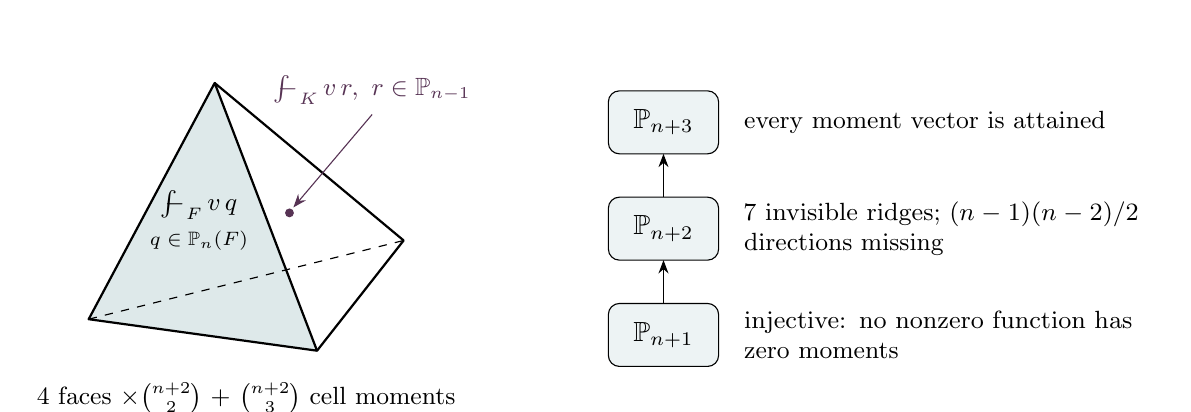
\begin{tikzpicture}[scale=1.0,line join=round]
 \coordinate (A) at (0,0); \coordinate (B) at (2.9,-0.4);
 \coordinate (C) at (4.0,1.0); \coordinate (D) at (1.6,3.0);
 \fill[inkteal!15] (A)--(B)--(D)--cycle;
 \draw[dashed] (A)--(C);
 \draw[thick] (A)--(B)--(D)--cycle; \draw[thick] (B)--(C)--(D);
 \node[font=\small] at (1.4,1.45) {\(\avg_F v\,q\)};
 \node[font=\scriptsize] at (1.4,1.0) {\(q\in\Pol_n(F)\)};
 \fill[inkplum] (2.55,1.35) circle (1.6pt);
 \draw[-{Stealth},inkplum] (3.6,2.6) node[above,font=\small]{\(\avg_K v\,r,\ r\in\Pol_{n-1}\)} -- (2.6,1.42);
 \node[font=\small,align=center] at (2.0,-1.0) {4 faces \(\times\binom{n+2}2\)\ +\ \(\binom{n+2}3\) cell moments};
 \begin{scope}[xshift=6.6cm,yshift=-0.6cm]
  \foreach \y/\lab/\txt in {0/{\(\Pol_{n+1}\)}/{injective: no nonzero function has zero moments},
     1.35/{\(\Pol_{n+2}\)}/{7 invisible ridges; \((n-1)(n-2)/2\) directions missing},
     2.7/{\(\Pol_{n+3}\)}/{every moment vector is attained}}{
   \draw[rounded corners,fill=inkteal!8] (0,\y) rectangle (1.4,\y+0.8);
   \node at (0.7,\y+0.4) {\lab};
   \node[anchor=west,font=\small,text width=5.2cm] at (1.6,\y+0.4) {\txt};}
  \draw[-{Stealth}] (0.7,0.8)--(0.7,1.35); \draw[-{Stealth}] (0.7,2.15)--(0.7,2.7);
 \end{scope}
\end{tikzpicture}
\caption{Left: the degrees of freedom on a tetrahedron. Right: what the
moments see in successive complete polynomial spaces
(Theorem~\ref{thm:main}). For \(n=3\) one direction is missing on
\(\Pol_5\), and it is supplied by the sextic \(\Delta_4\).}
\label{fig:overview}
\end{figure}

\begin{theorem}[Moment rank and minimum degree]
\label{thm:main}
For every tetrahedron \(K\) and every \(n\ge1\):
\begin{align}
 &\ker(\M_n|_{\Pol_{n+1}(K)})=\{0\},\label{eq:inj}\\
 &\dim\ker(\M_n|_{\Pol_{n+2}(K)})=7,\qquad
 \operatorname{rank}(\M_n|_{\Pol_{n+2}(K)})=\binom{n+5}3-7,\label{eq:kernel7}\\
 &c_n:=N_n-\operatorname{rank}(\M_n|_{\Pol_{n+2}(K)})=\frac{(n-1)(n-2)}2,
 \label{eq:deficit}\\
 &\M_n|_{\Pol_{n+3}(K)}\ \text{is surjective.}\label{eq:surj}
\end{align}
Consequently the smallest \(r\) for which a space satisfying
\eqref{eq:goal} exists inside \(\Pol_r(K)\) is \(r=n+2\) for \(n=1,2\) and
\(r=n+3\) for \(n\ge3\). Such spaces can be chosen invariant under vertex
relabelling and transported between tetrahedra by affine maps.
\end{theorem}

The kernel in \eqref{eq:kernel7} counts \emph{functions} invisible to
the moments; the number \(c_n\) in \eqref{eq:deficit} counts
\emph{moment directions} that \(\Pol_{n+2}\) cannot reach. They differ
because \(\dim\Pol_{n+2}\ne N_n\). The minimum-degree statement concerns
single-cell polynomial spaces satisfying \eqref{eq:goal}; it is not a
statement about all fourth-order Stokes elements.

\begin{table}[ht]
\centering
\caption{Consequences of Theorem~\ref{thm:main} \evid{proof; each entry
also checked by exact computation}.}
\label{tab:ranks}
\begin{tabular}{rrrrrrr}
\toprule
\(n\)&\(N_n\)&\(\dim\Pol_{n+1}\)&\(\dim\Pol_{n+2}\)&kernel&
\(\operatorname{rank}\) on \(\Pol_{n+2}\)&\(c_n\)\\
\midrule
1&13&10&20&7&13&0\\
2&28&20&35&7&28&0\\
3&50&35&56&7&49&1\\
4&80&56&84&7&77&3\\
5&119&84&120&7&113&6\\
6&168&120&165&7&158&10\\
\bottomrule
\end{tabular}
\end{table}

\begin{example}[The smallest cases]
\label{ex:small}
For \(n=1\) there are \(N_1=13\) moments: three per face and one
cell average. They are injective on the ten quadratics. On the twenty
cubics, the kernel is spanned by seven cubics such as
\(U_0=\lambda_0(5\lambda_0^2-5\lambda_0+1)\). This function vanishes on
\(F_0\). On a face \(F_j\), \(j\ne0\), Lemma~\ref{lem:aggregation} below reduces its
moments against \(1\), \(\lambda_0\) and either other coordinate to multiples of
\[
 \int_0^1 t(5t^2-5t+1)(1-t)\,dt,\quad
 \int_0^1 t^2(5t^2-5t+1)(1-t)\,dt,\quad
 \int_0^1 t(5t^2-5t+1)(1-t)^2\,dt,
\]
all of which are zero; the cell average reduces to the last integral. Since
\(20-7=13=N_1\), cubics reach every moment vector. For \(n=3\) the same
count gives \(56-7=49<50\): one direction is missing.
\end{example}

\section{The fourth-order obstruction and its sextic repair}
\label{sec:alternating}

This section does not use the kernel theorem. Put
\[
 \Delta_4=\prod_{0\le i<j\le3}(\lambda_j-\lambda_i),\qquad
 \Delta_3^{(i)}=\prod_{\substack{j<k\\ j,k\ne i}}(\lambda_k-\lambda_j),
 \qquad b_i=\prod_{j\ne i}\lambda_j,
\]
and define the signed cofactors
\begin{equation}
 \varepsilon_i=(-1)^i\Delta_3^{(i)}
 =-\frac{\Delta_4}{\prod_{j\ne i}(\lambda_i-\lambda_j)} .
 \label{eq:cofactor}
\end{equation}
The second expression follows from separating the factors of
\(\Delta_4\) that contain \(\lambda_i\): those with \(j<i\) give
\(\lambda_i-\lambda_j\) and the \(3-i\) factors with \(k>i\) give
\(\lambda_k-\lambda_i\). The alternating face functional is
\begin{equation}
 \mathcal A(v)=\sum_{i=0}^3\avg_{F_i}v\,\varepsilon_i\,ds .
 \label{eq:alternating}
\end{equation}
For \(n=3\) each term is a face moment, so \(\mathcal A\) is a linear
combination of the entries of \(\M_3v\).

\begin{lemma}[Sign rule]
\label{lem:sign}
For a permutation \(\sigma\) of \(\{0,1,2,3\}\) write
\((\sigma\lambda)_j=\lambda_{\sigma(j)}\) and \((v\circ\sigma)(\lambda)=v(\sigma\lambda)\).
Then \(\varepsilon_i(\sigma\lambda)=\operatorname{sgn}(\sigma)\,
\varepsilon_{\sigma(i)}(\lambda)\) and
\(\mathcal A(v\circ\sigma)=\operatorname{sgn}(\sigma)\mathcal A(v)\).
\end{lemma}

\begin{proof}
Since
\(\Delta_4(\sigma\lambda)=\operatorname{sgn}(\sigma)\Delta_4(\lambda)\)
and \(\prod_{j\ne i}(\lambda_{\sigma(i)}-\lambda_{\sigma(j)})=
\prod_{k\ne\sigma(i)}(\lambda_{\sigma(i)}-\lambda_k)\), the second form of
\eqref{eq:cofactor} gives the first identity. The substitution
\(\mu=\sigma\lambda\) is an affine automorphism of \(K\) that preserves
normalised measures and maps \(F_i\) onto \(F_{\sigma^{-1}(i)}\). Using the
first identity with \(\sigma^{-1}\),
\[
 \mathcal A(v\circ\sigma)=\sum_i\avg_{F_{\sigma^{-1}(i)}}v(\mu)\,
 \operatorname{sgn}(\sigma)\,\varepsilon_{\sigma^{-1}(i)}(\mu)\,ds
 =\operatorname{sgn}(\sigma)\mathcal A(v).\qedhere
\]
\end{proof}

\begin{proposition}[An explicit missing direction]
\label{prop:alternating}
\(\mathcal A\) vanishes on \(\Pol_5(K)\), and
\(\mathcal A(\Delta_4)=1/34650\). Hence the 50 moments \(\M_3\) are
linearly dependent on \(\Pol_5(K)\) and on every subspace of it.
\end{proposition}

\begin{proof}
Represent \(v\in\Pol_5\) by a homogeneous quintic in
\(\lambda_0,\dots,\lambda_3\), multiplying lower-degree parts by powers of
\(\sum_i\lambda_i=1\). Its antisymmetrisation
\(v^{\mathrm{alt}}=\frac1{24}\sum_\sigma\operatorname{sgn}(\sigma)v\circ\sigma\)
is an alternating homogeneous quintic. Setting \(\lambda_i=\lambda_j\)
shows that each \(\lambda_j-\lambda_i\) divides it; these linear forms are
pairwise coprime, so \(\Delta_4\), of degree six, divides it, and
\(v^{\mathrm{alt}}=0\). By Lemma~\ref{lem:sign},
\(\mathcal A(v)=\mathcal A(v^{\mathrm{alt}})=0\).

On \(F_i\), \eqref{eq:cofactor} with \(\lambda_i=0\) gives
\(\Delta_4|_{F_i}=-\varepsilon_i\prod_{j\ne i}(-\lambda_j)=\varepsilon_ib_i\),
so
\[
 \mathcal A(\Delta_4)=\sum_{i=0}^3\avg_{F_i}b_i\,(\Delta_3^{(i)})^2\,ds>0.
\]
On a triangle with barycentrics \(a,b,c\), a homogeneous polynomial \(h\)
of degree \(k\) satisfies
\(\avg_F h=\frac{2}{(k+2)!}\int_{\mathbb R_+^3}h(x)e^{-x_1-x_2-x_3}dx\),
because both sides equal \(2\alpha!\beta!\gamma!/(k+2)!\) on monomials.
With \(h=abc\,\Delta_3^2\) (\(k=9\)), the Andreief identity~\cite{For2019}
for the weight \(w(x)=xe^{-x}\) gives
\[
 \int_{\mathbb R_+^3}x_1x_2x_3\Delta_3(x)^2e^{-\sum x_i}dx
 =3!\det\bigl[(i+j+1)!\bigr]_{i,j=0}^{2}
 =6\det\begin{pmatrix}1&2&6\\2&6&24\\6&24&120\end{pmatrix}=144 .
\]
Thus each face contributes \(2\cdot144/11!=1/138600\), and four faces give
\(1/34650\).
\end{proof}

Changing basis, using nonmonomial quintics, or choosing other quintic
enrichments cannot help: \(\mathcal A\) vanishes on all of \(\Pol_5\).
This answers the question of Appendix~A of~\cite{BAJO2025} in the
negative. With Theorem~\ref{thm:main}, the rank of \(\M_3\) on \(\Pol_5\)
is exactly 49, so
\begin{equation}
 W_*:=\Pol_5(K)\oplus\operatorname{span}\{\Delta_4\},\qquad\dim W_*=57,
 \label{eq:Wstar}
\end{equation}
carries all 50 moments; seven kernel directions remain to be removed
(Section~\ref{sec:explicit}).

\section{The seven-dimensional kernel}
\label{sec:kernel}

We first show that at most seven polynomials of degree \(m=n+2\) are
invisible to the moments and then exhibit seven. Put
\(Z_m=\ker(\M_{m-2}|_{\Pol_m(K)})\), \(m\ge3\). Kernel dimensions are
affine invariants, so we work on
\(T=\{x\in\mathbb R^3:x_i\ge0,\ x_1+x_2+x_3\le1\}\) with \(\lambda_i=x_i\)
(\(i=1,2,3\)) and \(\lambda_0=1-x_1-x_2-x_3\).

\subsection{What vanishing moments say about derivatives}

\begin{lemma}[Gradient orthogonality]
\label{lem:gradient}
If \(p\in Z_m\), then \(\int_T(\partial_ip)q\,dx=0\) for all
\(q\in\Pol_{m-2}(T)\), \(i=1,2,3\). Moreover \(Z_m\cap\Pol_{m-1}(T)=\{0\}\);
hence \(p\mapsto\) (homogeneous part of degree \(m\)) is injective on \(Z_m\).
\end{lemma}

\begin{proof}
\(\int_T(\partial_ip)q=\sum_F\int_Fp\,q\,\eta_{F,i}\,ds-\int_Tp\,\partial_iq\),
with face tests of degree \(\le m-2=n\) and cell tests of degree
\(\le m-3=n-1\); both vanish. If also \(p\in\Pol_{m-1}\), then
\(\int_T|\nabla p|^2=\sum_F\int_Fp\,\partial_{\boldsymbol\eta}p-\int_Tp\,\Delta p=0\)
by the same degree count, so \(p\) is constant, and its face averages force
\(p=0\) (compare~\cite[Thm.~3.1]{YZ2021}).
\end{proof}

\subsection{A classical simplex operator}

Let \(\mathcal E=\sum_ix_i\partial_i\), \(\mathcal D=\sum_ix_i\partial_i^2+\sum_i\partial_i\)
and \(\mathcal L=\mathcal D-\mathcal E^2-3\mathcal E\). Then \(\mathcal E\)
multiplies a homogeneous polynomial of degree \(r\) by \(r\), \(\mathcal D\)
lowers degree by one, and
\begin{equation}
 \mathcal Lq=\operatorname{div}(C\nabla q),\qquad C(x)=\operatorname{diag}(x)-xx^{\mathsf T},
 \label{eq:divform}
\end{equation}
which is the uniform-weight simplex Jacobi operator~\cite[Eq.~(1.2)]{AX2013}.
Indeed \(\sum_i\partial_i(x_i\partial_iq)=\mathcal Dq\) and
\(\sum_i\partial_i(x_i\,\mathcal Eq)=3\mathcal Eq+\mathcal E^2q\).

\begin{lemma}[Orthogonal layers are eigenspaces]
\label{lem:jacobi}
If \(q\in\Pol_r(T)\), \(r\ge1\), is \(L^2(T)\)-orthogonal to \(\Pol_{r-1}(T)\), then
\(\mathcal Lq=-r(r+3)q\).
\end{lemma}

\begin{proof}
The flux \(C\nabla q\cdot\boldsymbol\eta\) vanishes on \(\partial T\): on
\(x_i=0\) the \(i\)-th component of \(C\nabla q\) is zero, and on
\(\sum x_i=1\) the sum of its components is \((1-\sum x_i)\,\mathcal Eq=0\).
So \(\mathcal L\) is symmetric in \(L^2(T)\). It maps \(\Pol_r\) to itself, with
leading part \(-r(r+3)\) times the leading part of \(q\), so
\(g=(\mathcal L+r(r+3))q\in\Pol_{r-1}\) and
\(\int_Tg^2=\int_Tq\,(\mathcal L+r(r+3))g=0\).
\end{proof}

\subsection{Compatibility leaves seven coefficient patterns}

\begin{lemma}[Upper bound]
\label{lem:upper}
For \(m\ge3\), \(\dim Z_m\le7\).
\end{lemma}

\begin{proof}
Write \(p=H+H'+(\text{degree}\le m-2)\) with \(H,H'\) homogeneous of
degrees \(m,m-1\). By Lemmas~\ref{lem:gradient} and~\ref{lem:jacobi},
\((\mathcal L+(m-1)(m+2))\partial_ip=0\). The terms of degree \(m-2\) give
\begin{equation}
 \mathcal D(\partial_iH)+2m\,\partial_iH'=0,\qquad i=1,2,3,
 \label{eq:nextdeg}
\end{equation}
since \((m-1)(m+2)-(m-2)(m+1)=2m\). Apply \(\partial_j\) to the \(i\)-th
equation and \(\partial_i\) to the \(j\)-th and subtract: the \(H'\) terms
cancel, and \([\partial_j,\mathcal D]=\partial_j^2\) gives
\begin{equation}
 \partial_i\partial_j(\partial_j-\partial_i)H=0,\qquad i\ne j.
 \label{eq:compat}
\end{equation}
Write \(H=\sum_{|\alpha|=m}c_\alpha x^\alpha/\alpha!\). Then
\eqref{eq:compat} says \(c_{\beta+e_i+2e_j}=c_{\beta+2e_i+e_j}\) for
\(|\beta|=m-3\): one unit of exponent may move between two positive
coordinates, keeping both positive, without changing the coefficient.
Such moves connect all exponents with the same support, so there is at
most one free coefficient per nonempty support \(S\subset\{1,2,3\}\), seven
in all. Lemma~\ref{lem:gradient} transfers the bound to \(Z_m\).
\end{proof}

The seven forms \((\sum_{i\in S}x_i)^m\), \(\varnothing\ne S\subset\{1,2,3\}\),
satisfy \eqref{eq:compat} and are independent: choose one monomial of
degree \(m\) with support exactly \(T\) for each \(T\); its coefficient in
\((\sum_{S}x_i)^m\), divided by the multinomial coefficient, is
\(\mathbf 1[T\subseteq S]\). Ordered by decreasing \(|T|\) this matrix is
unitriangular.

\subsection{Seven explicit ridge polynomials}

The integrals below all reduce to one variable by the following
classical property of the uniform distribution on a simplex.

\begin{lemma}[Integration along a barycentric sum]
\label{lem:aggregation}
Let \(S\) be a \(d\)-simplex with barycentrics \(\lambda_0,\dots,\lambda_d\),
let \(A\) be a nonempty proper subset of the labels, \(a=|A|\),
\(b=d+1-a\), \(s=\sum_{i\in A}\lambda_i\). For a multi-index \(\alpha\) and
an integrable \(\varphi\) on \([0,1]\),
\[
 \avg_S\varphi(s)\lambda^\alpha
 =c_\alpha\int_0^1\varphi(s)\,s^{a-1+|\alpha_A|}(1-s)^{b-1+|\alpha_{A^c}|}\,ds,
\]
with \(c_\alpha>0\) independent of \(\varphi\).
\end{lemma}

\begin{proof}
Under the normalised measure, \((\lambda_0,\dots,\lambda_d)\) is
Dirichlet\((1,\dots,1)\) distributed. By the aggregation property of the
Dirichlet law, \(s\) has density proportional to \(s^{a-1}(1-s)^{b-1}\),
and \(s\), \((\lambda_i/s)_{i\in A}\) and \((\lambda_i/(1-s))_{i\notin A}\)
are independent. Write
\(\lambda^\alpha=s^{|\alpha_A|}(1-s)^{|\alpha_{A^c}|}\prod_{i\in A}(\lambda_i/s)^{\alpha_i}
\prod_{i\notin A}(\lambda_i/(1-s))^{\alpha_i}\) and factor the expectation.
\end{proof}

Applied to a face \(F_j\) (a 2-simplex), the exponent of \(s\) drops by one
if \(j\in A\) and that of \(1-s\) drops by one if \(j\notin A\). We use the
Jacobi polynomials \(\J_r^{(\alpha,\beta)}\), for which
\(\J_r^{(\alpha,\beta)}(2t-1)\) is orthogonal on \([0,1]\) to
\(\Pol_{r-1}\) with weight \((1-t)^\alpha t^\beta\)~\cite[\S18.3]{DLMF},
and \(\J_r=\J_r^{(0,0)}\). A \emph{ridge} is a polynomial that depends on a
single affine combination of the coordinates. Define
\begin{equation}
 U_i=\lambda_i\,\J_{m-1}^{(1,1)}(2\lambda_i-1)\ (i=0,\dots,3),\qquad
 V_{0j}=\J_m\bigl(2(\lambda_0+\lambda_j)-1\bigr)\ (j=1,2,3).
 \label{eq:ridges}
\end{equation}

\begin{lemma}[Kernel basis]
\label{lem:ridges}
For \(m\ge3\), the seven polynomials \eqref{eq:ridges} form a basis of
\(Z_m\).
\end{lemma}

\begin{proof}
Use monomial tests \(\lambda^\alpha\) and Lemma~\ref{lem:aggregation}.
For \(U_i\) take \(A=\{i\}\) (\(a=1,b=3\)). On \(F_i\), \(U_i=0\). On \(F_j\),
\(j\ne i\), with \(|\alpha|\le m-2\), the moment is a multiple of
\(\int_0^1t(1-t)\J^{(1,1)}_{m-1}(2t-1)\,t^{\alpha_i}(1-t)^{|\alpha|-\alpha_i}dt=0\),
a test of degree \(\le m-2\). In the cell, \(|\alpha|\le m-3\) and the
weight \((1-t)^2\) leave a test \(t^{\alpha_i}(1-t)^{|\alpha|-\alpha_i+1}\)
of degree \(\le m-2\). For \(V_{0j}\) take \(A=\{0,j\}\) (\(a=b=2\)). Face weights
are \(s\) or \(1-s\) and face tests have degree \(\le m-2\); the cell weight
is \(s(1-s)\) and cell tests have degree \(\le m-3\). Either way \(\J_m\)
meets a polynomial of degree \(\le m-1\). Hence all seven lie in \(Z_m\).
Their leading parts are nonzero multiples of \(x_1^m,x_2^m,x_3^m,
(x_1+x_2+x_3)^m\) and \((x_1+x_2)^m,(x_1+x_3)^m,(x_2+x_3)^m\) (for
\(V_{0j}\), \(\lambda_0+\lambda_j=1-\sum_{k\ne j}x_k\) and the Legendre
parity \(\J_m(-t)=(-1)^m\J_m(t)\)), which are independent. Lemma~\ref{lem:upper}
completes the proof.
\end{proof}

\begin{remark}[Low-order precedents]
For \(m=3,4\) the vertex ridges are proportional to
\(5\lambda_i^3-5\lambda_i^2+\lambda_i\) and
\(14\lambda_i^4-21\lambda_i^3+9\lambda_i^2-\lambda_i\), which appear
in~\cite[Eqs.~(4), (11)]{CHZ2023}. The argument above concerns the combined
face and cell moments and gives completeness for every \(m\).
\end{remark}

\section{Sharp degree, minimal enrichment and symmetric elements}
\label{sec:construction}

\subsection{Degree \texorpdfstring{\(n+3\)}{n+3} suffices}

\begin{lemma}[Surjectivity on \(\Pol_{n+3}\)]
\label{lem:surj}
For every \(n\ge1\), \(\M_n|_{\Pol_{n+3}(K)}\) is surjective.
\end{lemma}

\begin{proof}
We show that the moment functionals are linearly independent on
\(\Pol_{n+3}\). Suppose
\(\sum_i\int_{F_i}v\,q_i\,ds+\int_Kv\,r\,dx=0\) for all \(v\in\Pol_{n+3}\),
with \(q_i\in\Pol_n(F_i)\), \(r\in\Pol_{n-1}(K)\). The test
\(v=\lambda_0\lambda_1\lambda_2\lambda_3r\) (degree \(\le n+3\)) vanishes on
\(\partial K\) and gives \(\int_K\lambda_0\cdots\lambda_3r^2=0\), so \(r=0\).
For a face \(F_i\), extend \(q_i\) to \(\tilde q_i\in\Pol_n(K)\); the test
\(v=b_i\tilde q_i\) vanishes on the other faces and gives
\(\int_{F_i}b_iq_i^2=0\), so \(q_i=0\).
\end{proof}

\begin{proof}[Proof of Theorem~\ref{thm:main}]
Lemma~\ref{lem:gradient} gives \eqref{eq:inj}, Lemma~\ref{lem:ridges}
and rank--nullity give \eqref{eq:kernel7}, and
\(N_n-\binom{n+5}3+7=(n-1)(n-2)/2\) gives \eqref{eq:deficit};
Lemma~\ref{lem:surj} is \eqref{eq:surj}. Degree \(n+1\) is too small since
\(N_n-\dim\Pol_{n+1}=n(n+2)>0\). If \(\M_n\) is surjective on \(\Pol_r\), extend
a basis of \(\Pol_{n+1}\) (on which \(\M_n\) is injective) by a complement of
\(\ker\M_n|_{\Pol_r}\) chosen to contain \(\Pol_{n+1}\); this gives
\eqref{eq:goal} in \(\Pol_r\). Surjectivity holds on \(\Pol_{n+2}\) exactly when
\(c_n=0\), that is \(n\le2\), and always on \(\Pol_{n+3}\). Invariance is
Proposition~\ref{prop:canonical}.
\end{proof}

\subsection{How many top-degree functions are needed}

\begin{corollary}[Minimal enrichment count]
\label{cor:minimal}
Let \(n\ge1\) and let \(V\) be any polynomial space satisfying
\eqref{eq:goal}. Then \(\dim\bigl((V+\Pol_{n+2})/\Pol_{n+2}\bigr)\ge c_n\):
every such space contains at least \((n-1)(n-2)/2\) independent directions
outside \(\Pol_{n+2}\). This number is attained by vertex-invariant spaces
inside \(\Pol_{n+3}\) (Theorem~\ref{thm:lean}).
\end{corollary}

\begin{proof}
Choose \(V'\subset V\) complementary to \(V\cap\Pol_{n+2}\). Then
\(\mathbb R^{N_n}=\M_n(V)\subset\M_n(\Pol_{n+2})+\M_n(V')\), so
\(N_n\le(N_n-c_n)+\dim V'\), and \(\dim V'=\dim((V+\Pol_{n+2})/\Pol_{n+2})\).
\end{proof}

\subsection{A numbering-free choice of complement}

Regard barycentric polynomials as functions on \(\sum_i\lambda_i=1\), and put
\begin{equation}
 \partial_{ij}=\frac{\partial}{\partial\lambda_i}-\frac{\partial}{\partial\lambda_j},
 \qquad
 a_B(u,v)=\avg_K\sum_{0\le i<j\le3}\partial_{ij}u\,\partial_{ij}v\,dx .
 \label{eq:aB}
\end{equation}
Tangent derivatives are well defined on the hyperplane and span its
tangent space, so \(a_B\) is positive semidefinite with kernel the
constants. It is invariant under vertex permutations and affine maps. On
a general tetrahedron it is a constant positive-definite metric applied to
the physical gradient, not the Euclidean Dirichlet form.

\begin{proposition}[Canonical complement]
\label{prop:canonical}
Let \(W\supset\Pol_{n+1}(K)\) be a vertex-invariant polynomial space with
\(\M_n|_W\) surjective, \(Z=\ker(\M_n|_W)\), and
\(V=\{v\in W:a_B(v,z)=0\ \forall z\in Z\}\). Then \(W=V\oplus Z\),
\(\dim V=N_n\), \(\Pol_{n+1}\subset V\), \(\M_n|_V\) is bijective, and \(V\) is
invariant under vertex relabelling and affine pullback.
\end{proposition}

\begin{proof}
No nonzero constant lies in \(Z\), so \(a_B\) is positive definite on \(Z\)
and \(W=V\oplus Z\); bijectivity and the dimension follow. For
\(p\in\Pol_{n+1}\), \(a_B(p,z)=\avg_K\nabla z\cdot G\nabla p\) with a constant
symmetric matrix \(G\); integrating by parts places on \(z\) face tests
\(G\nabla p\cdot\boldsymbol\eta\in\Pol_n(F)\) and the cell test
\(\operatorname{div}(G\nabla p)\in\Pol_{n-1}\), so \(a_B(p,z)=0\). Invariance
holds because \(Z\) and \(a_B\) are invariant.
\end{proof}

With \(W=\Pol_{n+2}\) for \(n=1,2\) this gives numbering-free elements of
minimal degree, answering the concern of Remark~3.6 of~\cite{BAJO2025};
they differ from the non-symmetric spaces listed there. For \(n\ge3\),
\(W=\Pol_{n+3}\) works but uses many top-degree directions. The next
subsection removes this waste.

\subsection{Lean symmetric elements for every order}

The symmetric group \(\mathfrak S_4\) acts on polynomials by relabelling
vertices and on moment vectors by permuting faces and transforming the
tests; \(\M_n\) is equivariant. Hence the space of missing directions
\(C_n=\mathbb R^{N_n}/\M_n(\Pol_{n+2})\) is an \(\mathfrak S_4\)-module of
dimension \(c_n\).

\begin{theorem}[Lean symmetric elements]
\label{thm:lean}
For every \(n\ge3\) there is a vertex-invariant space \(E_n\subset\Pol_{n+3}(K)\)
with \(\dim E_n=c_n\) and \(E_n\cap\Pol_{n+2}=\{0\}\) such that
\(W_n=\Pol_{n+2}\oplus E_n\) satisfies: \(\M_n|_{W_n}\) is surjective and
\(\ker(\M_n|_{W_n})=Z_{n+2}\). The canonical complement \(V_n\subset W_n\) of
Proposition~\ref{prop:canonical} satisfies \eqref{eq:goal}, is invariant,
and has exactly \(c_n\) independent directions outside \(\Pol_{n+2}\), the
minimum of Corollary~\ref{cor:minimal}.
\end{theorem}

\begin{proof}
Let \(Q\) be the \(L^2(K)\)-orthogonal complement of \(\Pol_{n+2}\) in
\(\Pol_{n+3}\); it is invariant because normalised \(L^2\) is. The composite
\(Q\to\mathbb R^{N_n}\to C_n\) is equivariant, and surjective by
Lemma~\ref{lem:surj}. By Maschke's theorem~\cite{Serre1977} its kernel has
an invariant complement \(E_n\subset Q\), mapped isomorphically onto \(C_n\).
Then \(\M_n(W_n)=\M_n(\Pol_{n+2})+\M_n(E_n)=\mathbb R^{N_n}\), and
\(\dim\ker=\dim\Pol_{n+2}+c_n-N_n=7\); the kernel contains \(Z_{n+2}\), so equals
it. Since \(Z_{n+2}\subset\Pol_{n+2}\), \(V_n+\Pol_{n+2}=W_n\).
\end{proof}

The theorem is existential. The next result identifies the module and
suggests an explicit choice.

\begin{proposition}[The missing directions as a representation]
\label{prop:character}
For \(n\ge3\), \(C_n\cong\mathrm{sgn}\otimes\mathrm{Sym}^{n-3}(\mathrm{std})\),
where \(\mathrm{std}\) is the three-dimensional standard representation of
\(\mathfrak S_4\). The space \(\Delta_4\Pol_{n-3}(K)\) modulo \(\Pol_{n+2}\) is
isomorphic to the same module.
\end{proposition}

\begin{proof}
By Theorem~\ref{thm:main}, \(C_n\) equals, as a virtual module,
\(\mathbb R^{N_n}-\Pol_{n+2}+Z_{n+2}\). The characters of the face part
(induced from the vertex stabiliser), of \(\Pol_{n-1}\) and \(\Pol_{n+2}\)
(Molien series of the permutation action on \(\lambda_0,\dots,\lambda_3\)),
and of \(Z_{n+2}\) (vertex ridges permute like vertices; pair ridges permute
like the three bipartitions, with the sign \((-1)^{n+2}\) when the two parts
are exchanged) have rational generating functions in \(n\). Explicitly, for
\(g\in\mathfrak S_4\) let \(f_g(t)=\prod_{\text{cycles }\gamma}(1-t^{|\gamma|})^{-1}\)
(cycles of \(g\) on the four vertices), let \(\phi_g\) be the number of fixed
vertices, let \(f'_g\) be the same product over the cycles of \(g\) on the
three vertices other than one fixed vertex, and let \(\beta^\pm_g\) be the
numbers of bipartitions \(\{A,A^c\}\) into pairs fixed by \(g\) with
\(gA=A\) (\(+\)) or \(gA=A^c\) (\(-\)). Then
\[
 \sum_{n\ge1}\chi_{C_n}(g)\,t^n
 =\phi_g\bigl(f'_g(t)-1\bigr)+t f_g(t)-\frac{f_g(t)-[f_g]_{\le2}(t)}{t^2}
 +\frac{(\phi_g+\beta^+_g)\,t}{1-t}-\frac{\beta^-_g\,t}{1+t},
\]
where \([f]_{\le2}\) is the Taylor polynomial of degree two; the five terms
are the face part, \(\Pol_{n-1}\), \(-\Pol_{n+2}\), the vertex ridges plus
the bipartitions kept, and those exchanged (sign \((-1)^{n+2}\)). The
character of \(\mathrm{sgn}\otimes\mathrm{Sym}^{n-3}(\mathrm{std})\) has
generating function \(\operatorname{sgn}(g)\,t^3(1-t)f_g(t)\), because the
permutation representation is \(\mathrm{triv}\oplus\mathrm{std}\). With
\((\phi_g,\beta^+_g,\beta^-_g)\) and \(\operatorname{sgn}(g)t^3(1-t)f_g(t)\) equal to
\[
\begin{array}{lll}
 e:&(4,3,0),&t^3/(1-t)^3,\\
 (01):&(2,1,0),&-t^3/((1-t)^2(1+t)),\\
 (01)(23):&(0,1,2),&t^3/((1-t)(1+t)^2),\\
 (012):&(1,0,0),&t^3/(1-t^3),\\
 (0123):&(0,0,1),&-t^3/((1+t)(1+t^2)),
\end{array}
\]
the two sides agree as rational functions on each class
\evid{exact symbolic computation; script \texttt{verify\_lean\_element.py}}.
For example, on the identity both sides reduce to \(\sum_n\binom{n-1}2t^n\).
For the second statement, \(\Pol_r(K)\) is identified with homogeneous
polynomials of degree \(r\) in \(\lambda_0,\dots,\lambda_3\), and \(\Pol_{r-1}\)
with multiples of \(e=\sum_i\lambda_i\). Since \(e\) does not divide
\(\Delta_4\), \(\Delta_4f\) is a multiple of \(e\) only when \(f\) is, so
\(\Delta_4\Pol_{n-3}/(\Delta_4\Pol_{n-3}\cap\Pol_{n+2})\cong
\mathrm{sgn}\otimes\mathrm{Sym}^{n-3}(V/\langle e\rangle)\) with
\(V/\langle e\rangle\cong\mathrm{std}\). Its dimension is
\(\binom{n}{3}-\binom{n-1}3=c_n\).
\end{proof}

\begin{conjecture}[Explicit lean enrichment]
\label{conj:lean}
For every \(n\ge3\), \(E_n=\Delta_4\Pol_{n-3}(K)\) (modulo \(\Pol_{n+2}\))
can be used in Theorem~\ref{thm:lean}, that is,
\(\M_n\) is surjective on \(\Pol_{n+2}+\Delta_4\Pol_{n-3}\).
\end{conjecture}

This holds for \(n=3\) by Proposition~\ref{prop:alternating} \evid{proof}
and for \(n=3,\dots,8\) by exact computation: the spaces have dimensions
\(57,87,126,175,235,307\) and moment rank \(N_n\) \evid{exact computation}.
For \(n=3,4\) the module is irreducible, so by Schur's lemma a single
nonzero value suffices.

\begin{example}[An explicit lean element for \(n=4\)]
\label{ex:n4}
Let \(\Pi_6\) be the \(a_B\)-orthogonal projection of \(\Pol_6\) onto the
complement of \(Z_6\). The space
\[
 V_4^\flat=\Pi_6(\Pol_6)+\operatorname{span}\{\lambda_0\Delta_4,\lambda_1\Delta_4,
 \lambda_2\Delta_4,\lambda_3\Delta_4\}
\]
has dimension \(77+4-1=80\) (the four products sum to \(\Delta_4\in\Pol_6\)),
contains \(\Pol_5\), is unisolvent for the 80 moments \(\M_4\) and is
vertex-invariant; it uses three degree-7 directions, the minimum
\(c_4=3\) \evid{exact computation}. The products \(\lambda_i\Delta_4\) are
\(a_B\)-orthogonal to \(Z_6\) by Schur's lemma, since they span
\(\mathrm{sgn}\oplus(\mathrm{sgn}\otimes\mathrm{std})\) while \(Z_6\) contains
only trivial, standard and two-dimensional components; this is also
checked exactly. Similarly, for \(n=5\) the space
\(\Pi_7(\Pol_7)+\Delta_4\Pol_2\) has dimension 119, contains \(\Pol_6\), is
unisolvent for \(\M_5\) and is invariant \evid{exact computation}.
\end{example}

\subsection{The 50-dimensional fourth-order element}
\label{sec:explicit}

For \(n=3\), \(m=5\), the kernel of \(\M_3\) on \(W_*\) in \eqref{eq:Wstar}
is \(Z_5\) (an element with a nonzero \(\Delta_4\) component would have
\(\mathcal A\ne0\)). Moreover \(a_B(\Delta_4,p)=0\) for \(p\in\Pol_5\): by
invariance the pairing equals the pairing of \(\Delta_4\) with the
antisymmetrisation of \(p\), which is zero. Hence:

\begin{corollary}[One-sextic fourth-order element]
\label{cor:fourth}
The space
\begin{equation}
 V_3^*(K)=\{p\in\Pol_5(K):a_B(p,z)=0\ \forall z\in Z_5\}\oplus
 \operatorname{span}\{\Delta_4\}
 \label{eq:V3}
\end{equation}
has dimension 50, contains \(\Pol_4(K)\), is unisolvent for \(\M_3\), and is
invariant under vertex relabelling and affine maps. Every polynomial space
satisfying \eqref{eq:goal} for \(n=3\) has degree at least six and at least
one direction outside \(\Pol_5\), so \(V_3^*\) is minimal in both senses.
\end{corollary}

This is the minimal-rank repair: it uses the least possible number of
sextic directions. We do not classify all fourth-order spaces.

\emph{Gram matrix.} Let
\(\kappa=(U_0,U_1,U_2,U_3,V_{01},V_{02},V_{03})\) with \(m=5\), and put
\(f(t)=t\J_4^{(1,1)}(2t-1)\), \(g(s)=\J_5(2s-1)\). From
\(\partial_{ab}U_i=f'(\lambda_i)(\mathbf 1[a=i]-\mathbf 1[b=i])\) and
\(\partial_{ab}V_A=g'(s_A)(\mathbf 1[a\in A]-\mathbf 1[b\in A])\):
\begin{itemize}
\item \(a_B(U_i,U_i)=3\avg f'(\lambda_i)^2\) and
 \(a_B(U_i,U_j)=-\avg f'(\lambda_i)f'(\lambda_j)\) (\(i\ne j\)), one-
 and two-variable integrals against the densities \(3(1-t)^2\) and
 \(6(1-t-u)\) (Lemma~\ref{lem:aggregation}), equal to \(225/11\) and
 \(-5/11\);
\item \(a_B(V_A,V_A)=4\avg g'(s)^2=4\int_0^16s(1-s)g'(s)^2ds=720/11\),
 by \(\int_{-1}^1(1-x^2)\J_5'(x)^2dx=2\cdot30/11\); distinct pair ridges
 share two crossing edges with opposite signs, so are \(a_B\)-orthogonal;
\item \(a_B(U_i,V_A)=\pm2\avg f'(\lambda_i)g'(s_A)=\pm60/11\), with \(+\)
 if \(i\in A\).
\end{itemize}
The values \(225/11\), \(-5/11\) and \(60/11\) are evaluated in exact
arithmetic. Thus
\begin{equation}
\begin{gathered}
 \Gamma=\frac1{11}\begin{pmatrix}230I_4-5J_4&60S\\60S^{\mathsf T}&720I_3\end{pmatrix},
 \qquad
 \Gamma^{-1}=11\begin{pmatrix}I_4/210&-S/2520\\-S^{\mathsf T}/2520&23I_3/15120\end{pmatrix},
 \\
 S=\begin{pmatrix}1&1&1\\1&-1&-1\\-1&1&-1\\-1&-1&1\end{pmatrix},
\end{gathered}
 \label{eq:gram}
\end{equation}
where \(J_4\) is the all-ones matrix; the inverse follows from
\(S^{\mathsf T}S=4I_3\), \(SS^{\mathsf T}=4I_4-J_4\), \(J_4S=0\).

\emph{Projection.} For \(q\in\Pol_5\) let
\(\Pi q=q-\kappa^{\mathsf T}\Gamma^{-1}(a_B(\kappa_1,q),\dots,a_B(\kappa_7,q))^{\mathsf T}\).
This is the identity on \(\Pol_4\) and maps \(\Pol_5\) onto the first summand
of \eqref{eq:V3}.

\begin{proposition}[A 14-monomial basis]
\label{prop:fourteen}
Let \(Q_{14}\) be the quintics \(x_1^ax_2^bx_3^c\) with \((a,b,c)\) in
\{(0,1,4), (0,2,3), (0,3,2), (1,0,4), (1,1,3), (1,2,2), (1,3,1),
(1,4,0), (2,0,3), (2,1,2), (2,2,1), (2,3,0), (3,0,2), (3,2,0)\}. A basis of
\(\Pol_4\), the fourteen \(\Pi q\) (\(q\in Q_{14}\)) and \(\Delta_4\) form a
basis of \(V_3^*(K)\).
\end{proposition}

\begin{proof}
The seven excluded quintic exponents \((5,0,0)\), \((0,5,0)\), \((0,0,5)\), \((4,1,0)\),
\((4,0,1)\), \((0,4,1)\), \((3,1,1)\) have one exponent for each nonempty support
\(S\subset\{1,2,3\}\). Modulo \(\Pol_4\) and \(\operatorname{span}Q_{14}\), the
leading form \((\sum_{i\in S}x_i)^5\) of the ridge with support \(S\) has
coefficients on these seven monomials forming a lower triangular matrix with
diagonal \((1,1,1,5,5,5,20)\) (the multinomial coefficients). Hence
\(\Pol_4+\operatorname{span}Q_{14}+Z_5=\Pol_5\), so
\(\Pi(\Pol_4+\operatorname{span}Q_{14})\) is the 49-dimensional first summand.
\end{proof}

An exact certificate confirms the full \(50\times50\) moment matrix of this
basis (determinant \(-1/(2^{174}3^{112}5^{65}7^{46}\,11)\)). The determinant is
tiny because of scaling, not because of near-dependence; see
Section~\ref{sec:implementation} for a well-conditioned basis.

\section{Triangles and higher-dimensional simplices}
\label{sec:dimension}

On a \(d\)-simplex \(K_d\), let \(\M_{d,n}\) consist of all facet moments
against \(\Pol_n\) and cell moments against \(\Pol_{n-1}\), \(n\ge1\), \(m=n+2\).
Then \(N_{d,n}=(d+1)\binom{n+d-1}{d-1}+\binom{n+d-1}{d}\). Put
\(k(d,m)=\sum_{r=1}^{\min(d,m)}\binom dr\).

\begin{theorem}[Kernel on a \(d\)-simplex]
\label{thm:ddim}
For \(d\ge2\), \(\M_{d,n}\) is injective on \(\Pol_{m-1}(K_d)\),
\(\dim\ker(\M_{d,n}|_{\Pol_m})=k(d,m)\), and it is surjective on \(\Pol_{n+d}\).
\end{theorem}

\begin{proof}
Lemma~\ref{lem:gradient} holds verbatim. With
\(\mathcal L_d=\mathcal D-\mathcal E^2-d\mathcal E=\operatorname{div}(C\nabla\cdot)\),
orthogonal layers satisfy \(\mathcal L_dq=-r(r+d)q\), and the degree-\((m-2)\)
terms give \(\mathcal D\partial_iH+(2m+d-3)\partial_iH'=0\), hence
\eqref{eq:compat}. A degree-\(m\) monomial has at most \(\min(d,m)\) variables,
so there are at most \(k(d,m)\) free coefficients. For the lower bound, take a
nonempty proper label set \(A\), \(a=|A|\), \(b=d+1-a\), \(s=\sum_{A}\lambda_i\),
and define \(R_A=\J_m^{(b-2,a-2)}(2s-1)\) if \(a,b\ge2\), \(R_A=s\,
\J_{m-1}^{(d-2,1)}(2s-1)\) if \(a=1\) (and the complementary rule if \(b=1\)).
By Lemma~\ref{lem:aggregation}, facet and cell weights are the Jacobi weight
times \(s\), \(1-s\) or \(s(1-s)\), and the test degrees are low enough, as in
Lemma~\ref{lem:ridges}. For \(S\subset\{1,\dots,d\}\), \(1\le|S|\le\min(d,m)\),
take \(A\) to be \(S\) (or the complement \(\{0\}\) when \(S=\{1,\dots,d\}\));
the leading part of \(R_A\) is a nonzero multiple of \((\sum_Sx_i)^m\), and the
unitriangular support argument gives independence. Surjectivity on
\(\Pol_{n+d}\) follows as in Lemma~\ref{lem:surj} with the cell bubble (degree
\(d+1\)) and facet bubbles (degree \(d\)).
\end{proof}

\begin{proposition}[Missing directions in every dimension]
\label{prop:cdn}
\(c(d,n):=N_{d,n}-\operatorname{rank}(\M_{d,n}|_{\Pol_{n+2}})\) equals
\[
 c(d,n)=\sum_{r=3}^{\min(d,n)}\binom dr\Bigl[(r-2)\binom n{r-1}-\binom n{r-2}+1\Bigr].
\]
Every term is positive. Hence \(c(d,n)=0\) if \(d=2\) or \(n\le2\), and
\(c(d,n)>0\) if \(d\ge3\) and \(n\ge3\). For example \(c(3,n)=(n-1)(n-2)/2\),
\(c(d,3)=\binom d3\), and \(c(4,n)=(n-2)(n+5)(2n-3)/6\) for \(n\ge2\)
(\(c(4,1)=0\)).
\end{proposition}

\begin{proof}
Write \(h_r=\binom{r+d-1}{d-1}\) for the number of degree-\(r\) monomials in
\(d\) variables. From \(\binom{n+1+d}{d}=\binom{n+d-1}{d}+h_n+h_{n+1}\),
\[
 c(d,n)=d\,h_n-h_{n+1}-h_{n+2}+k(d,n+2).
\]
Counting monomials by support size gives \(h_r=\sum_{t\ge1}\binom dt\binom{r-1}{t-1}\)
(\(r\ge1\)). Using \(d\binom dt=t\binom dt+(t+1)\binom d{t+1}\) and Pascal's rule,
\(d\,h_n=\sum_t\binom dt\,t\binom n{t-1}\). Collecting coefficients of
\(\binom dt\) and using \(\binom{n+1}{t-1}=\binom n{t-1}+\binom n{t-2}\) gives
the bracket \((t-2)\binom n{t-1}-\binom n{t-2}+\mathbf 1[t\le n+2]\), which is
zero for \(t=1,2,n+1,n+2\) and for \(t>n+2\). For \(3\le t\le n\),
\((t-2)\binom n{t-1}=\binom n{t-2}\frac{(t-2)(n-t+2)}{t-1}\ge\binom n{t-2}\)
because \((t-2)(n-t+2)\ge2(t-2)\ge t-1\), so the bracket is at least one.
\end{proof}

\begin{corollary}[Triangles]
\label{cor:2d}
For edge moments against \(\Pol_n\) and cell moments against \(\Pol_{n-1}\) on a
triangle, the kernel on \(\Pol_{n+2}\) is three-dimensional and the moments are
surjective on \(\Pol_{n+2}\) for every \(n\ge1\). A unisolvent space containing
\(\Pol_{n+1}\) is obtained by adding \(n\) functions of degree \(n+2\).
\end{corollary}

This is why triangular constructions in the spirit of~\cite{FS1983,MT2005,BS2007}
can stay one degree above the reproduced polynomials at every order, while on
tetrahedra the extra degree becomes necessary at fourth order. In dimension
\(d\ge3\) Theorem~\ref{thm:ddim} and Proposition~\ref{prop:cdn} give, for
\(n\ge3\), a minimum degree between \(n+3\) and \(n+d\).

\begin{conjecture}[Sharp degree in every dimension]
\label{conj:ddim}
For every \(d\ge3\) and \(n\ge1\), \(\M_{d,n}\) is surjective on \(\Pol_{n+3}(K_d)\).
Hence the minimum degree is \(n+2\) for \(n\le2\) and \(n+3\) for \(n\ge3\).
\end{conjecture}

\begin{table}[ht]
\centering
\caption{Evidence for Conjecture~\ref{conj:ddim} \evid{exact computation}.
Full row rank modulo the prime \(2^{61}-1\) implies full rank over
\(\mathbb Q\), so each ``yes'' is a certificate of surjectivity.}
\label{tab:ddim}
\begin{tabular}{rlll}
\toprule
\(d\)&\(n\) checked&\(c(d,n)\) on \(\Pol_{n+2}\)&surjective on \(\Pol_{n+3}\)\\
\midrule
2&1--6&0&yes\\
3&1--6&0,0,1,3,6,10&yes\\
4&1--5&0,0,4,15,35&yes\\
5&1--4&0,0,10,45&yes\\
6&1--3&0,0,20&yes\\
\bottomrule
\end{tabular}
\end{table}

The ranks on \(\Pol_{n+2}\) in Table~\ref{tab:ddim} agree with
Theorem~\ref{thm:ddim}. The bubble proof of Lemma~\ref{lem:surj} uses that cell
and face bubbles have degrees \(4\) and \(3\), which is special to \(d=3\); a
proof of Conjecture~\ref{conj:ddim} will need a different argument.

\section{Stokes consequences}
\label{sec:stokes}

These results apply the established nonconforming framework
of~\cite{CR1973,BAJO2025}; we state them to fix hypotheses. Let
\(\Omega\subset\mathbb R^3\) be a bounded connected Lipschitz polyhedron, and
\(\mathcal T_h\) a conforming shape-regular family of affine tetrahedral
meshes. Transport a reference space \(V_n\) from Theorem~\ref{thm:main} (for
example \(V_3^*\) or a lean space) to each cell. Let \(X_h\) consist of
piecewise functions in \(V_n(K)\) whose jumps on interior faces, and traces on
boundary faces, are orthogonal to \(\Pol_n(F)\); put \(\mathbf X_h=X_h^3\) and
\(Q_h=\{q\in L^2_0(\Omega):q|_K\in\Pol_n(K)\}\). The broken seminorm
\(|v|_{1,h}^2=\sum_K\|\nabla v\|_{0,K}^2\) is a norm on \(X_h\) (zero gradients give
piecewise constants, which shared face averages and the boundary condition
force to vanish).

\begin{lemma}[Fortin operator]
\label{lem:fortin}
Let \(I_h\) match the moments \eqref{eq:moments} on every cell. There is
\(C_I\), independent of \(h\), with \(|I_hv|_{1,h}\le C_I|v|_{1,\Omega}\) for
\(v\in H^1_0(\Omega)\), and
\(\sum_K\int_K\operatorname{div}(\mathbf v-I_h\mathbf v)q_h=0\) for
\(\mathbf v\in H^1_0(\Omega)^3\), \(q_h\in Q_h\).
\end{lemma}

\begin{proof}
On the reference cell the moments are \(H^1\)-continuous (trace theorem) and
the inverse into the polynomial space is bounded; constants are reproduced, so
a Poincaré argument and affine scaling give the stability bound. Integration
by parts writes \(\int_K\operatorname{div}(\mathbf v-I_K\mathbf v)q_h\) as face
moments against \(q_h\boldsymbol\eta_K\) (degree \(\le n\)) and cell moments
against \(\nabla q_h\) (degree \(\le n-1\)), all zero.
\end{proof}

\begin{corollary}[Discrete inf-sup]
If \(\beta_\Omega>0\) is the continuous inf-sup constant, then
\(\inf_{q_h}\sup_{\mathbf v_h}\frac{\sum_K\int_Kq_h\operatorname{div}\mathbf v_h}
{|\mathbf v_h|_{1,h}\|q_h\|_0}\ge\beta_\Omega/C_I\).
\end{corollary}

For viscosity \(\nu>0\) and \(\mathbf f\in L^2(\Omega)^3\), the discrete problem
uses \(a_h(\mathbf u,\mathbf v)=\nu\sum_K\int_K\nabla\mathbf u:\nabla\mathbf v\) and
\(b_h(\mathbf v,q)=-\sum_K\int_Kq\operatorname{div}\mathbf v\), with exact
integration. This is the vector-Laplacian form; a symmetric-gradient form
would need a discrete Korn inequality, which we do not study.

\begin{proposition}[Energy-order convergence]
\label{prop:error}
If \(\mathbf u\in H^{n+2}(\Omega)^3\cap H^1_0\) and \(p\in H^{n+1}(\Omega)\cap L^2_0\), then
\(|\mathbf u-\mathbf u_h|_{1,h}+\|p-p_h\|_0\le C h^{n+1}
(\|\mathbf u\|_{n+2}+\|p\|_{n+1})\), with \(C\) depending on \(n\), \(\Omega\),
\(\nu\) and shape regularity. For \(V_3^*\) this is fourth order.
\end{proposition}

\begin{proof}
Interpolation reproduces \(\Pol_{n+1}\), which gives the approximation term.
The consistency error consists of face terms \(\int_F(\sigma\boldsymbol\eta_F)\cdot
[\mathbf v_h]\) with \(\sigma=\nu\nabla\mathbf u-pI\); since jumps are orthogonal to
\(\Pol_n(F)\), subtracting a face projection of \(\sigma\boldsymbol\eta_F\) and using
trace and Poincaré inequalities bounds it by
\(Ch^{n+1}(\nu\|\mathbf u\|_{n+2}+\|p\|_{n+1})|\mathbf v_h|_{1,h}\). The
nonconforming saddle-point Strang estimate~\cite[Ch.~5]{BBF2013} combines this
with coercivity and the inf-sup bound.
\end{proof}

No claim is made about pressure robustness~\cite{JLMNR2017}, curved cells,
or \(p\)-uniform constants.

\section{A numerical Stokes test}
\label{sec:numerics}

All results in this section are \evid{numerical}. We used \(V_3^*\) on the unit
cube, split into \(N^3\) subcubes of six Kuhn tetrahedra each, with
\(\nu=1\), the exact solution
\(\mathbf u=\operatorname{curl}(\phi,\phi,\phi)\),
\(\phi=\sin^2(\pi x)\sin^2(\pi y)\sin^2(\pi z)\), and
\(p=\cos(\pi x)\cos(\pi y)\cos(\pi z)\). The mean-zero pressure condition was
imposed by a Lagrange multiplier. Polynomial products were integrated
exactly: stiffness, divergence and mass terms with a collapsed
Gauss--Jacobi (Stroud) rule with 8 points per direction (512 points,
exact to degree 15), and face moments with the corresponding triangle rule
with 5 points per direction (exact to degree 9). The non-polynomial load
\((\mathbf f,\mathbf v_h)\) and all error norms were computed with the same
fixed 512-point degree-15 rule on every cell, without adaptivity or a
tolerance; we did not separately quantify this quadrature error. The
system was solved by a sparse direct solver.

\begin{table}[ht]
\centering
\caption{Errors and observed rates for \(V_3^*\) with discontinuous \(\Pol_3\)
pressure \evid{numerical}. \(h\) is the largest edge length.}
\label{tab:stokes}
\begin{tabular}{rrrrrrrr}
\toprule
\(N\)&\(h\)&velocity DOFs&\(|\mathbf u-\mathbf u_h|_{1,h}\)&rate&
\(\|\mathbf u-\mathbf u_h\|_0\)&rate&\(\|p-p_h\|_0\) (rate)\\
\midrule
1&1.732&360&4.638&--&0.2791&--&0.9318 (--)\\
2&0.866&3600&0.6501&2.84&0.02457&3.51&0.1414 (2.72)\\
3&0.5774&12960&0.1239&4.09&0.003009&5.18&0.02268 (4.51)\\
4&0.4330&31680&0.04119&3.83&7.508e-4&4.83&0.007201 (3.99)\\
5&0.3464&63000&0.01727&3.90&2.520e-4&4.89&0.002924 (4.04)\\
\bottomrule
\end{tabular}
\end{table}

The coarsest meshes are pre-asymptotic. The computed rates are consistent
with, but do not by themselves prove, the fourth-order estimate. From \(N=3\) on, the broken
\(H^1\) velocity error and the pressure error decrease at rates close to
four, as Proposition~\ref{prop:error} predicts, and the \(L^2\) velocity error
at a rate approaching five. The discrete inf-sup constant, computed as the
square root of the smallest positive generalised eigenvalue of
\(BA^{-1}B^{\mathsf T}q=\beta^2Mq\) on mean-zero pressures, is
\(0.4017,\ 0.3817,\ 0.3743,\ 0.3702\) for \(N=1,\dots,4\). These values
are consistent with the mesh-independent bound of the Fortin argument
(Lemma~\ref{lem:fortin}); four meshes cannot establish mesh independence. On a single element shrinking by halves, moment
interpolation of a smooth function showed rates 4.94 in \(L^2\) and 3.97 in the
\(H^1\) seminorm, and a random quartic was reproduced to relative error below
\(10^{-12}\).

\section{Implementation remarks}
\label{sec:implementation}

\emph{Consistent face bases.} Neighbouring cells must use the same test
functions on a shared face. We write the face tests in the face's three
barycentric coordinates ordered by global vertex index; since \(V_3^*\) and the
lean spaces are invariant under relabelling, the local space does not depend
on the cell's vertex order, and no further transformation of degrees of
freedom is needed (compare the general discussion in~\cite{SDRW2022}).

\emph{Well-conditioned basis.} Exact determinants are a poor guide to
conditioning. On the reference tetrahedron the \(50\times50\) moment matrix
has 2-norm condition number about \(6.6\times10^7\) for the monomial-type basis
of Proposition~\ref{prop:fourteen} with monomial tests, and about \(7.6\) for an
\(L^2\)-orthonormal basis of \(V_3^*\) with orthonormal face and cell tests
\evid{numerical}. We therefore recommend computing an orthonormal basis of
\(V_3^*\) once, in barycentric terms, and the nodal (degree-of-freedom dual)
basis from it; because the moments are normalised, the same nodal basis
serves every affine cell. The reference stiffness matrix in that nodal basis
has condition number about \(7.2\times10^2\) on the nonconstant subspace.

\emph{Quadrature.} Stiffness integrals need degree 8 for the quintic part and
degree 10 for products involving \(\Delta_4\); face moments need degree 9. Since
only one basis function is sextic, the higher-degree rule can be restricted to
its row and column.

\emph{Counts.} Per velocity component the element has 10 degrees of freedom on
each face and 10 in each cell; the cell ones can be condensed statically. On
Kuhn meshes this is about 30 per cell per component (about 20 after
condensation), with 20 pressure unknowns per cell. Conforming \(\Pol_4\)
Lagrange velocities need fewer unknowns but are not inf-sup stable with
discontinuous \(\Pol_3\) pressures on general meshes; split-mesh conforming
elements~\cite{SV1985,GN2014a} and virtual elements~\cite{CGM2016} are the
natural alternatives to compare in a dedicated study, which we have not done.

\section{Conclusion and open problems}

The face-and-cell moments that make nonconforming Stokes elements inf-sup stable
see all of \(\Pol_{n+1}\), miss exactly seven polynomials of degree \(n+2\), and
see everything in degree \(n+3\). On tetrahedra this forces degree \(n+3\) from
fourth order on, explains why the quintic search of~\cite{BAJO2025} could not
succeed, and yields numbering-free elements with the fewest possible top-degree
functions. Open problems: a proof of Conjectures~\ref{conj:lean}
and~\ref{conj:ddim}; other moment patterns, such as facet tests one degree below
the shape functions as in~\cite{BCS2026}; discrete Korn inequalities and
pressure-robust reconstructions for this family; and \(p\)-robust constants.

\section*{Statements}

\noindent\textbf{Use of AI tools.} Generative AI tools were used in developing
the arguments, the verification code and the text. All mathematical statements
were checked by the author, and the proofs, exact computations and numerical
results are reported with the evidence labels used throughout. Responsibility
for the content rests with the author.

\noindent\textbf{Data and code availability.} The exact verifiers, the
numerical Stokes code and their deterministic outputs are available in the
accompanying archive, doi:\href{https://doi.org/10.5281/zenodo.23565002}{10.5281/zenodo.23565002}, with source at \url{https://github.com/ipitchford/tetrahedral-moment-stokes-elements}. A single script
regenerates every certificate byte for byte and checks it against published
SHA-256 sums.

\noindent\textbf{Competing interests.} None.

\begin{thebibliography}{99}\small

\bibitem{AX2013} R.~Aktaş and Y.~Xu, Sobolev orthogonal polynomials on a simplex,
\emph{Int. Math. Res. Not.} 2013(13) (2013), 3087--3131.
\href{https://doi.org/10.1093/imrn/rns141}{doi:10.1093/imrn/rns141};
\href{https://arxiv.org/abs/1111.2994}{arXiv:1111.2994}.

\bibitem{AFW2006} D.~N.~Arnold, R.~S.~Falk and R.~Winther, Finite element exterior
calculus, homological techniques, and applications, \emph{Acta Numer.} 15 (2006),
1--155. \href{https://doi.org/10.1017/S0962492906210018}{doi:10.1017/S0962492906210018}.

\bibitem{BAJO2025} L.~Balazi, G.~Allaire, P.~Jolivet and P.~Omnes, Inf-sup stable
non-conforming finite elements on tetrahedra with second- and third-order accuracy,
\emph{Numer. Methods Partial Differential Equations} 41(6) (2025), e70057.
\href{https://doi.org/10.1002/num.70057}{doi:10.1002/num.70057}. Open version:
\href{https://hal.science/hal-04541809v3}{hal-04541809v3}.

\bibitem{BS2007} Á.~Baran and G.~Stoyan, Gauss--Legendre elements: a stable, higher
order non-conforming finite element family, \emph{Computing} 79(1) (2007), 1--21.
\href{https://doi.org/10.1007/s00607-007-0219-1}{doi:10.1007/s00607-007-0219-1}.

\bibitem{BR1985} C.~Bernardi and G.~Raugel, Analysis of some finite elements for the
Stokes problem, \emph{Math. Comp.} 44(169) (1985), 71--79.
\href{https://doi.org/10.1090/S0025-5718-1985-0771031-7}{doi:10.1090/S0025-5718-1985-0771031-7}.

\bibitem{BBF2013} D.~Boffi, F.~Brezzi and M.~Fortin, \emph{Mixed Finite Element
Methods and Applications}, Springer, 2013.
\href{https://doi.org/10.1007/978-3-642-36519-5}{doi:10.1007/978-3-642-36519-5}.

\bibitem{BCS2026} N.-E.~Bohne, P.~Ciarlet, Jr. and S.~Sauter, Crouzeix--Raviart
elements on simplicial meshes in \(d\) dimensions, \emph{Found. Comput. Math.}
(2026), online first.
\href{https://doi.org/10.1007/s10208-026-09741-1}{doi:10.1007/s10208-026-09741-1};
\href{https://arxiv.org/abs/2407.04361}{arXiv:2407.04361}.

\bibitem{CGM2016} A.~Cangiani, V.~Gyrya and G.~Manzini, The nonconforming virtual
element method for the Stokes equations, \emph{SIAM J. Numer. Anal.} 54(6) (2016),
3411--3435. \href{https://doi.org/10.1137/15M1049531}{doi:10.1137/15M1049531};
\href{https://arxiv.org/abs/1608.01210}{arXiv:1608.01210}.

\bibitem{CHZ2023} W.~Chen, J.~Hu and M.~Zhang, Nonconforming finite element methods
of order two and order three for the Stokes flow in three dimensions, \emph{J. Sci.
Comput.} 97(1) (2023), art.~1.
\href{https://doi.org/10.1007/s10915-023-02317-z}{doi:10.1007/s10915-023-02317-z};
\href{https://arxiv.org/abs/2212.11748}{arXiv:2212.11748}.

\bibitem{CDS2018} P.~Ciarlet, Jr., C.~F.~Dunkl and S.~A.~Sauter, A family of
Crouzeix--Raviart finite elements in 3D, \emph{Anal. Appl.} 16(5) (2018), 649--691.
\href{https://doi.org/10.1142/S0219530518500070}{doi:10.1142/S0219530518500070};
\href{https://arxiv.org/abs/1703.03224}{arXiv:1703.03224}.

\bibitem{CR1973} M.~Crouzeix and P.-A.~Raviart, Conforming and nonconforming finite
element methods for solving the stationary Stokes equations I, \emph{RAIRO Anal.
Numér.} 7(R3) (1973), 33--75.
\href{https://doi.org/10.1051/m2an/197307R300331}{doi:10.1051/m2an/197307R300331}.

\bibitem{DLMF} NIST Digital Library of Mathematical Functions, \S18.3,
\url{https://dlmf.nist.gov/18.3}.

\bibitem{For2019} P.~J.~Forrester, Meet Andréief, Bordeaux 1886, and Andreev,
Kharkov 1882--1883, \emph{Random Matrices Theory Appl.} 8(2) (2019), 1930001.
\href{https://doi.org/10.1142/S2010326319300018}{doi:10.1142/S2010326319300018};
\href{https://arxiv.org/abs/1806.10411}{arXiv:1806.10411}.

\bibitem{FS1983} M.~Fortin and M.~Soulié, A non-conforming piecewise quadratic
finite element on triangles, \emph{Int. J. Numer. Methods Eng.} 19(4) (1983),
505--520. \href{https://doi.org/10.1002/nme.1620190405}{doi:10.1002/nme.1620190405}.

\bibitem{GN2014a} J.~Guzmán and M.~Neilan, Conforming and divergence-free Stokes
elements in three dimensions, \emph{IMA J. Numer. Anal.} 34(4) (2014), 1489--1508.
\href{https://doi.org/10.1093/imanum/drt053}{doi:10.1093/imanum/drt053}.

\bibitem{GN2014b} J.~Guzmán and M.~Neilan, Conforming and divergence-free Stokes
elements on general triangular meshes, \emph{Math. Comp.} 83(285) (2014), 15--36.
\href{https://doi.org/10.1090/S0025-5718-2013-02753-6}{doi:10.1090/S0025-5718-2013-02753-6}.

\bibitem{JLMNR2017} V.~John, A.~Linke, C.~Merdon, M.~Neilan and L.~G.~Rebholz, On
the divergence constraint in mixed finite element methods for incompressible flows,
\emph{SIAM Rev.} 59(3) (2017), 492--544.
\href{https://doi.org/10.1137/15M1047696}{doi:10.1137/15M1047696}.

\bibitem{MT2005} G.~Matthies and L.~Tobiska, Inf-sup stable non-conforming finite
elements of arbitrary order on triangles, \emph{Numer. Math.} 102(2) (2005),
293--309. \href{https://doi.org/10.1007/s00211-005-0648-8}{doi:10.1007/s00211-005-0648-8}.

\bibitem{ST2023} S.~Sauter and C.~Torres, On the inf-sup stability of
Crouzeix--Raviart Stokes elements in 3D, \emph{Math. Comp.} 92(341) (2023),
1033--1059. \href{https://doi.org/10.1090/mcom/3793}{doi:10.1090/mcom/3793};
\href{https://arxiv.org/abs/2205.00062}{arXiv:2205.00062}.

\bibitem{SV1985} L.~R.~Scott and M.~Vogelius, Norm estimates for a maximal right
inverse of the divergence operator in spaces of piecewise polynomials, \emph{RAIRO
Modél. Math. Anal. Numér.} 19(1) (1985), 111--143.
\href{https://doi.org/10.1051/m2an/1985190101111}{doi:10.1051/m2an/1985190101111}.

\bibitem{SDRW2022} M.~W.~Scroggs, J.~S.~Dokken, C.~N.~Richardson and G.~N.~Wells,
Construction of arbitrary order finite element degree-of-freedom maps on polygonal
and polyhedral cell meshes, \emph{ACM Trans. Math. Softw.} 48(2) (2022), 1--23.
\href{https://doi.org/10.1145/3524456}{doi:10.1145/3524456}.

\bibitem{Serre1977} J.-P.~Serre, \emph{Linear Representations of Finite Groups},
Springer, 1977. \href{https://doi.org/10.1007/978-1-4684-9458-7}{doi:10.1007/978-1-4684-9458-7}.

\bibitem{YZ2021} X.~Ye and S.~Zhang, A \(P_{k+2}\) polynomial lifting operator on
polygons and polyhedrons, \emph{Appl. Math. Lett.} 116 (2021), 107033.
\href{https://doi.org/10.1016/j.aml.2021.107033}{doi:10.1016/j.aml.2021.107033};
\href{https://arxiv.org/abs/2009.13604}{arXiv:2009.13604}.

\end{thebibliography}
\end{document}
